\documentclass[UTF8]{ctexart}
\title{CS229 Lecture notes}
\author{原作者:Andrew Ng(吴恩达)}
\author{翻译:CycleUser}
\author{排版:HappyUncle}
\date{\today}
\usepackage{graphics}
\usepackage{amssymb}
\usepackage{amsmath}

\begin{document}
	
	\paragraph{}
	\begin{description}
		\item[CS229 Lecture notes]
		\item[原作者:Andrew Ng(吴恩达)]
		\item[翻译:CycleUser]
		\item[排版:HappyUncle]
		\item[\today]
	\end{description}
	
	\part*{监督学习(Supervised learning)}
	
	\paragraph{}
		咱们先来聊几个使用监督学习来解决问题的实例。假如咱们有一个数据集,里面的数据是俄勒冈州波特兰市的 47 套房屋的面积和价格:
	
	\begin{figure}[h]
		\centering
		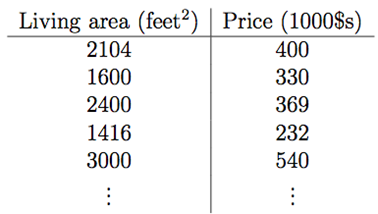
\includegraphics{images/screenshot001}
	\end{figure}
	
	\paragraph{}
		这些数据来投个图吧:
	
	\begin{figure}[h]
		\centering
		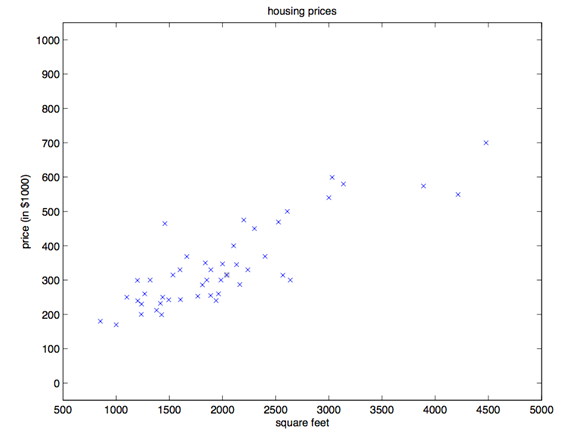
\includegraphics{images/screenshot002}
	\end{figure}
	
	\paragraph{}
		这里要先规范一下符号和含义,这些符号以后还要用到,咱们假设 $x^{i}$ 表示 “输入的” 变量值(在这个例子中就是房屋面积),也可以叫做输入特征;然后咱们用 $y^{i}$ 来表示“输出值”,或者称之为目标变量,这个例子里面就是房屋价格。这样的一对 $(x^{(i)},y^{(j)})$ 就称为一组训练样本,然后咱们用来让机器来学习的数据集,就是一个长度为 $m$的训练样本的列表$\{(x^{(i)},y^{(j)});i=1,...,m\}$也叫做一个训练集。另外一定注意,这里的上标 “$(i)$” 只是作为训练集的索引记号,和数学乘方没有任何关系,千万别误解了。另外我们还会用大写的 $ \mathcal{X} $ 来表示 输入值的空间,大写的 $ \mathcal{Y} $ 表示输出值的空间。在本节的这个例子中,输入输出的空间都是实数域,所以 $ \mathcal{X = Y = R} $。
	
		然后再用更加规范的方式来描述一下监督学习问题,我们的目标是,给定一个训练集,来让机器学习一个函数 $ h: \mathcal{X} \mapsto \mathcal{Y} $,让 $ h(x) $ 能是一个与对应的真实 $ y $ 值比较接近的评估值。由于一些历史上的原因,这个函数 $ h $ 就被叫做\textbf{假设}(英文hypothesis)。用一个图来表示的话,这个过程大概就是下面这样:
	
	\begin{figure}[h]
		\centering
		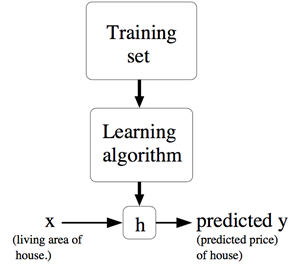
\includegraphics{images/screenshot003}
	\end{figure}
	
	\paragraph{}
		如果我们要预测的目标变量是连续的,比如在咱们这个房屋价格-面积的案例中,这种学习问题就被称为\textbf{回归}问题。如果 y 只能取一小部分的离散的值(比如给定房屋面积,咱们要来确定这个房子是一个住宅还是公寓),这样的问题就叫做\textbf{分类}问题。
	
	\clearpage
	
	\part{线性回归}
	
	\paragraph{}
		为了让我们的房屋案例更有意思,咱们稍微对数据集进行一下补充,增加上每一个房屋的卧室数目
	
	\begin{figure}[h]
		\centering
		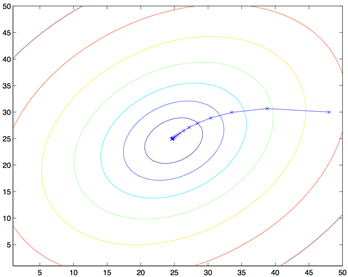
\includegraphics{images/screenshot004}
	\end{figure}
	
	\paragraph{}
		现在,输入特征 $ x $ 就是在 $ \mathbb{R}^{2} $ 范围取值的一个二维向量了。例如 $x _{1}^{(i)}$ 就是训练集中第 $i$ 个房屋的面积,而 $x_{2}^{(i)}$ 就是训练集中第 $i$ 个房屋的卧室数目。(通常来说,设计一个学习算法的时候,选择那些输入特征都取决于你,所以如果你不在波特兰收集房屋信息数据,你也完全可以选择包含其他的特征,例如房屋是否有壁炉,卫生间的数量啊等等。关于特征筛选的内容会在后面的章节进行更详细的介绍,不过目前来说就暂时先用给定的这两个特征了。)
		
		要进行这个监督学习,咱们必须得确定好如何在计算机里面对这个\textbf{函数/假设} $h$ 进行表示。咱们现在刚刚开始,就来个简单点的,咱们把 $y$ 假设为一个以 $x$ 为变量的线性函数:
		
		\[ h_{\theta}(x) = \theta_{0} + \theta_{1}x_{1} + \theta_{2}x_{2} \]
		
		这里的$ \theta_{i} $是\textbf{参数}(也可以叫做\textbf{权重}),是从 $\mathcal{X}$ 到$ \mathcal{Y} $的线性函数映射的空间参数。在不至于引起混淆的情况下,咱们可以把$h_{\theta}(x)$ 里面的 $\theta$ 省略掉,就简写成 $h(x)$。另外为了简化公式,咱们还设 $x_{0} = 1$(这个也是$\textbf{截距项intercept term}$)。这样简化之后就有了:
		
		\[ h(x) = \sum_{i=0}^{n} \theta_{i}x_{i} = \theta^{T}x \]
		
		等式的最右边的$ \theta $和$ x $都是向量,等式中的$ n $ 是输入变量的个数(不包括$x_{0}$ )。
		
		现在,给定了一个训练集了,咱们怎么来挑选/学习参数$\theta$呢?一个看上去比较合理的方法就是让 $h(x)$ 尽量逼近 $y$,至少对咱已有的训练样本能适用。用公式的方式来表示的话,就要定义一个函数,来衡量对于每个不同的 $\theta$ 值,$h(x^{(i)})$ 与对应的 $y^{(i)}$ 的距离。这样用如下的方式定义了一个 \textbf{成本函数} (\textbf{cost function}): 
		
		\[ J(\theta) = \frac{1}{2} \sum_{i=1}^{m}(h_{\theta}(x^{(i)}) - y^{(i)})^2 \]
		
		如果之前你接触过线性回归,你会发现这个函数和常规\textbf{最小二乘法}拟合模型中的最小二乘法成本函数非常相似。不管之前接触过没有,咱们都接着往下进行,以后就会发现这是一个更广泛的算法家族中的一个特例。
		
		\section{最小均方算法(LMS algorithm)}
		
		\paragraph{}
		我们希望选择一个能让 $J(\theta)$ 最小的 $\theta$ 值。怎么做呢,咱们先用一个搜索的算法,从某一个对 $\theta$ 的“初始猜测值”,然后对 $\theta$ 值不断进行调整,来让 $J(\theta)$ 逐渐变小,最好是直到我们能够达到一个使 $J(\theta)$ 最小的 $\theta$。具体来说,咱们可以考虑使用\textbf{梯度下降法(gradient descent algorithm)},这个方法就是从某一个 $\theta$ 的初始值开始,然后逐渐重复更新:
		
		\[ \theta_{j} := \theta_{j} - \alpha\frac{\partial}{\partial\theta_{j}}J(\theta) \]
		
		\textbf{注:}本文中“:= ” 表示的是计算机程序中的一种赋值操作,是把等号右边的计算结果赋值给左边的变量,“$ a := b $” 就表示用 $ b $ 的值覆盖$ a $ 原有的值。要注意区分,如果写的是“$ a = b $” 则表示的是判断二者相等的关系。(译者注:在 Python 中,单个等号 = 就是赋值,两个等号 ==  表示相等关系的判断。) 
		
		(上面的这个更新要同时对应从 $0$ 到 $ n $ 的所有$ j $ 值进行。)这里的 $ \alpha$ 也称为学习速率。这个算法是很自然的,逐步重复朝向 $ J $ 降低最快的方向移动。
		
		要实现这个算法,咱们需要解决等号右边的导数项。首先来解决只有一组训练样本 $ (x, y) $ 的情况,这样就可以忽略掉等号右边对 $ J $ 的求和项目了。公式就简化下面这样:
		
		\begin{align*}
			 \frac{\partial}{\partial\theta_{j}}J(\theta)  &=  \frac{\partial}{\partial\theta_{j}} \frac{1}{2}(h_{\theta}(x)-y)^2 \\
			   &= 2 \cdot \frac{1}{2}(h_{\theta}(x)-y) \cdot  \frac{\partial}{\partial\theta_{j}}(h_{\theta}(x)-y) \\
			   &= (h_{\theta}(x)-y) \cdot \frac{\partial}{\partial\theta_{j}}( \sum_{i=0}^{n}\theta_{i}x_{i} - y) \\
			   &= (h_{\theta}(x)-y) x_{j}
		\end{align*}
		
		对单个训练样本,更新规则如下所示:
		
		\[ \theta_{j} := \theta_{j} + \alpha(y^{(i)} - h_{\theta}(x^{(i)}))x_{j}^{(i)} \]
		
		
		这个规则也叫 LMS 更新规则 (LMS 是 “least mean squares” 的缩写,意思是最小均方),也被称为 Widrow-Hoff 学习规则。这个规则有几个看上去就很自然直观的特性。例如,更新的大小与$ (y^{(i)} - h_{\theta}(x^{(i)})) $成正比;另外,当我们遇到训练样本的预测值与 $ y^{(i)} $ 的真实值非常接近的情况下,就会发现基本没必要再对参数进行修改了;与此相反的情况是,如果我们的预测值 $ h_{\theta}(x^{(i)}) $ 与 $ y^{(i)} $ 的真实值有很大的误差(比如距离特别远),那就需要对参数进行更大地调整。
		
		
		当只有一个训练样本的时候,我们推导出了 LMS 规则。当一个训练集有超过一个训练样本的时候,有两种对这个规则的修改方法。第一种就是下面这个算法:
		
		\par 重复直到收敛\{

			\begin{center}
				$ \theta_{j} := \theta_{j} + \alpha \sum_{i=1}^{m} (y^{(i)} - h_{\theta}(x^{(i)}))x_{j}^{(i)}$
				(对于每一个$j$)
			\end{center}
		\par\}
		
		读者很容易能证明,在上面这个更新规则中求和项的值就是 $ \partial J(\theta) / \partial \theta_{j} $ (这是因为对 $J$ 的原始定义)。所以这个更新规则实际上就是对原始的成本函数 $J$ 进行简单的梯度下降。这一方法在每一个步长内检查所有整个训练集中的所有样本,也叫做批量梯度下降法(batch gradient descent)。这里要注意,因为梯度下降法容易被局部最小值影响,而我们要解决的这个线性回归的优化问题只能有一个全局的而不是局部的最优解;因此,梯度下降法应该总是收敛到全局最小值(假设学习速率 $\alpha$ 不设置的过大)。$J$ 是一个凸的二次函数。下面是一个样例,其中对一个二次函数使用了梯度下降法来找到最小值。
		
		\begin{figure}[h]
			\centering
			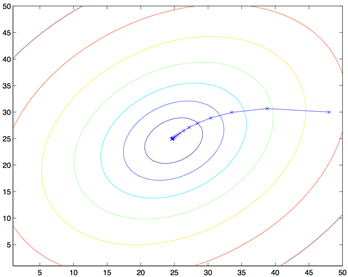
\includegraphics{images/screenshot004}
		\end{figure}
		
		上图的椭圆就是一个二次函数的轮廓图。图中还有梯度下降法生成的规矩,初始点位置$在(48,30)$。图中的画的 $x$ (用直线连接起来了)标记了梯度下降法所经过的 $ \theta $ 的可用值。
		
		对咱们之前的房屋数据集进行批量梯度下降来拟合 $ \theta $,把房屋价格当作房屋面积的函数来进行预测,我们得到的结果是  $ \theta_{0} = 71.27 $,  $ \theta_{1} = 0.1345 $。如果把 $ h_{\theta}(x) $ 作为一个定义域在 $x$ 上的函数来投影,同时也投上训练集中的已有数据点,会得到下面这幅图:
		
		\begin{figure}[h]
			\centering
			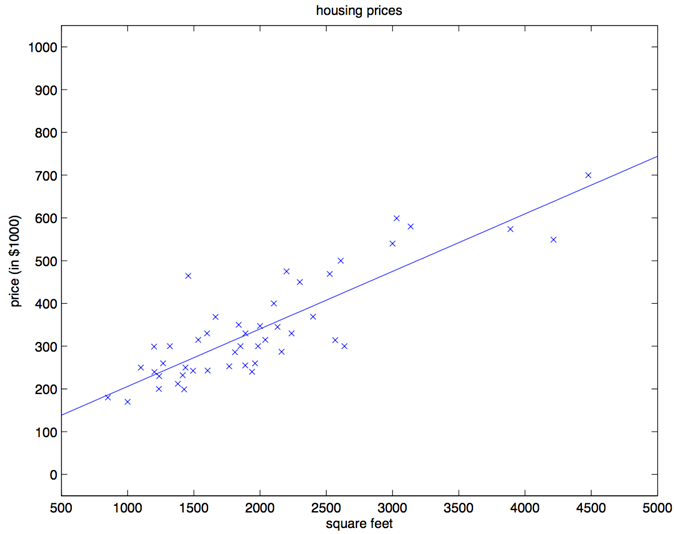
\includegraphics{images/screenshot005}
		\end{figure}
		
		如果在数据集中添加上卧室数目作为输入特征,那么得到的结果就是$ \theta_{0} = 89.60$, $\theta_{1} = 0.1392$, $\theta_{2} = \--8.738$。
		
		这个结果就是用批量梯度下降法来获得的。此外还有另外一种方法能够替代批量梯度下降法,这种方法效果也不错。如下所示:
		
		\par Loop \{
			\par \setlength \parindent{2em} for i=1:m,\{ 
				\begin{center}
					$ \theta_{j} := \theta_{j} + \alpha (y^{(i)} - h_{\theta}(x^{(i)}))x_{j}^{(i)}$
				(对于每一个$j$)
				\end{center}
			\par \setlength \parindent{2em} \}
		\par \}
		
		在这个算法里,我们对整个训练集进行了循环遍历,每次遇到一个训练样本,根据每个单一训练样本的误差梯度来对参数进行更新。这个算法叫做随机梯度下降法(stochastic gradient descent),或者叫增量梯度下降法(incremental gradient descent)。批量梯度下降法要在运行第一步之前先对整个训练集进行扫描遍历,当训练集的规模 m 变得很大的时候,因此引起的性能开销就很不划算了;随机梯度下降法就没有这个问题,而是可以立即开始,对查询到的每个样本都进行运算。通常情况下,随机梯度下降法查找到足够接近最低值的 $ \theta $ 的速度要比批量梯度下降法更快一些。(也要注意,也有可能会一直无法收敛(converge)到最小值,这时候 $ \theta $ 会一直在 $ J( \theta )$ 最小值附近震荡;不过通常情况下在最小值附近的这些值大多数其实也足够逼近了,足以满足咱们的精度要求,所以也可以用。当然更常见的情况通常是我们事先对数据集已经有了描述,并且有了一个确定的学习速率$\alpha$,然后来运行随机梯度下降,同时逐渐让学习速率$\alpha$随着算法的运行而逐渐趋于 $ \theta $ ,这样也能保证我们最后得到的参数会收敛到最小值,而不是在最小值范围进行震荡。) 由于以上种种原因,通常更推荐使用的都是随机梯度下降法,而不是批量梯度下降法,尤其是在训练用的数据集规模大的时候。 
		
		\section{法方程(The normal equations) }
		上文中的梯度下降法是一种找出 J 最小值的办法。然后咱们聊一聊另一种实现方法,这种方法寻找起来简单明了,而且不需要使用迭代算法。这种方法就是,我们直接利用找对应导数为 $ \theta $ 位置的 $ \theta_{j} $,这样就能找到 J 的最小值了。我们想实现这个目的,还不想写一大堆代数公式或者好几页的矩阵积分,所以就要介绍一些做矩阵积分的记号。
		
		\subsection{矩阵导数(Matrix derivatives)}
		假如有一个函数 $ f : R^{m×n} \longrightarrow R $ 从 $ m * n $ 大小的矩阵映射到实数域,那么就可以定义当矩阵为 $A$ 的时候有导函数$ f $ 如下所示:
		\[ \nabla_{A}f(A)=\begin{bmatrix}
		\dfrac{\partial f}{\partial A_{11}} & \cdots & \dfrac{\partial f}{\partial A_{1n}}\\
		\vdots & \ddots & \vdots \\
		\dfrac{\partial f}{\partial A_{m1}} & \cdots & \dfrac{\partial f}{\partial A_{mn}}\\
		\end{bmatrix}  \]
		
		因此,这个梯度 $ \nabla_{A}f(A) $  本身也是一个 $m*n$ 的矩阵,其中的第 $(i,j)$ 个元素是 $ \partial f / \partial A_{ij} $ 。例如,假如 $ A=\begin{bmatrix}
		A_{11} & A_{12} \\ A_{21} & A_{22} \\
		\end{bmatrix} $ 是一个 2*2 矩阵,然后给定的函数 $f : R^{2×2} \longrightarrow R$ 为:
		
		\[ f(A) = \frac{3}{2}A_{11} + 5A^{2}_{12} + A_{21}A_{22} \]
		
		这里面的 $ A_{ij} $ 表示的意思是矩阵 $A$ 的第$(i,j)$ 个元素。然后就有了梯度:
		
		\[ \nabla_{A}f(A) = \begin{bmatrix}
		\frac{3}{2} & 10A_{12} \\ a_{22} & A_{21}
		\end{bmatrix} \]
		
		然后咱们还要引入 $trace$ 求迹运算,简写为 $\mathrm{tr}$。对于一个给定的 $n*n$ 方形矩阵 $A$,它的迹定义为对角项和:
		
		\[ \mathrm{tr}A= \sum^{n}_{i=1}A_{ii} \]
		
		假如 $a$ 是一个实数,实际上 $a$ 就可以看做是一个 $1*1$ 的矩阵,那么就有 $a$ 的迹 $\mathrm{tr} a = a$。(如果你之前没有见到过这个“运算记号”,就可以把 $A$ 的迹看成是 $\mathrm{tr}(A)$,或者理解成为一个对矩阵 $A$ 进行操作的 $trace$ 函数。不过通常情况都是写成不带括号的形式更多一些。) 
		如果有两个矩阵 $A$ 和 $B$,能够满足 $AB$ 为方阵,$trace$ 求迹运算就有一个特殊的性质: $trAB = trBA$. (自己想办法证明!)在此基础上进行推论,就能得到类似下面这样的等式关系: 
		
		\[ trABC = trCAB = trBCA  \]
		\[ trABCD = trDABC = trCDAB = trBCDA \]
		
		下面这些和求迹运算相关的等量关系也很容易证明。其中 $A$ 和 $B$ 都是方形矩阵,$a$ 是一个实数: 
		
		\[ \mathrm{tr}A = \mathrm{tr}A^{T} \]
		\[ \mathrm{tr}(A+B) = \mathrm{tr}A + \mathrm{tr}B\]
		\[ \mathrm{tr}aA = a\mathrm{tr}A \]
		
		接下来咱们就来在不进行证明的情况下提出一些矩阵导数(其中的一些直到本节末尾才用得上)。另外要注意等式(4) $ A $必须是非奇异方形矩阵(non-singular square matrices),而 $|A|$ 表示的是矩阵 $A$ 的行列式。那么我们就有下面这些等量关系: 
		
		\begin{align}
			\nabla_{A}\mathrm{tr}AB &= B^{T} \\
			\nabla_{A^{T}}f(A) &= (\nabla_{A}f(A))^{T} \\
			\nabla_{A}\mathrm{tr}ABA^{T}C &= CAB + C^{T}AB^{T} \\
			\nabla_{A}|A| &= |A|(A^{-1})^{T} 
		\end{align}
		
		为了让咱们的矩阵运算记号更加具体,咱们就详细解释一下这些等式中的第一个。加入我们有俩一个确定的矩阵 $B \in R^{n×m}$  (注意顺序,是$n*m$,这里的意思也就是 $B$ 的元素都是实数,$B$的形状是 $n*m$ 的一个矩阵),那么接下来就可以定义一个函数 $f: Rm×n \longrightarrow R$ ,对应这里的就是 $f(A) = trAB$。这里要注意,这个矩阵是有意义的,因为如果 $A ∈ Rm×n $, 那么 $AB$ 就是一个方阵,是方阵就可以应用 $trace$ 求迹运算;因此,实际上 $f$ 映射的是从 $Rm×n$ 到实数域 $R$。这样接下来就可以使用矩阵导数来找到$ \nabla_{A}f(A) $ ,这个导函数本身也是一个 $m*n$ 的矩阵。上面的等式$(1)$ 表明了这个导数矩阵的第 $(i, j)$个元素等同于 $BT$ (($B$的转置)的第 $(i, j)$ 个元素,或者更直接表示成 $Bji$。 
		上面等式$(1-3)$ 都很简单,证明就都留给读者做练习了。等式$(4)$需要用逆矩阵的伴随矩阵来推导出。
		注:假如咱们定义一个矩阵 $A′$,它的第$ (i, j) $个元素是$ (−1)i+j $与矩阵 $A$ 去除 第 $i$ 行 和 第 $j$ 列 之后的行列式的乘积,则可以证明有$A−1 = (A′)T /|A|$。(你可以检查一下,比如在 $A$ 是一个 $2*2$ 矩阵的情况下看看 $A-1$ 是什么样的,然后以此类推。如果你想看看对于这一类结果的证明,可以参考一本中级或者高级的线性代数教材,比如Charles Curtis, 1991, Linear Algebra, Springer。)这也就意味着 $A′ = |A|(A−1)T$ 。此外,一个矩阵 $A$ 的行列式也可以写成 $|A| = AijA′$ 。因为$ (A′)ij $不依赖$ Aij $(通过定义也能看出来),这也就意味着$(∂/∂Aij)|A| = A′ij $,综合起来也就得到上面的这个结果了。
		
		
	
	
		
\end{document}